% *********************************************************************
% © 2026 Jeremy Sylvestre
%
% Permission is granted to copy, distribute and/or modify this document
% under the terms of the GNU Free Documentation License, Version 1.3 or
% any later version published by the Free Software Foundation; with no
% Invariant Sections, no Front-Cover Texts, and no Back-Cover Texts. A
% copy of the license is included in the appendix entitled “GNU Free
% Documentation License” that appears in the output document of this
% PreTeXt source code. All trademarks™ are the registered® marks of
% their respective owners.
%
% *********************************************************************
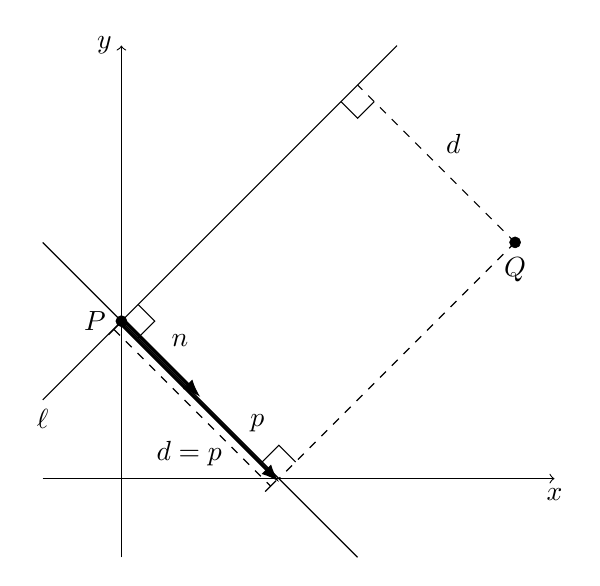
\begin{tikzpicture}[
	vector/.style={-latex,very thick},
	point/.style={circle,draw,very thin,fill,inner sep=0pt,minimum size=4pt},
	% scale=0.75
]
	% projection
	\coordinate (P) at (0,2);
	\coordinate (Q) at (5,3);
	\coordinate (n) at (1,1);
	\coordinate (p) at (2,0);
	\coordinate (foot) at (3,5);

	\draw[->] (-1,0) to (5.5,0) node[below] {$x$};
	\draw[->] (0,-1) to (0,5.5) node[left] {$y$};

	% parallel to (1,1)
	\draw[thin] (-1,1) to node[below,at start] {$\ell$} (3.5,5.5);
	% parallel to (1,-1)
	\draw[thin] (-1,3) to (3,-1);

	\node[point] at (P) [label=left:$P$] {};
	\node[point] at (Q) [label=below:$Q$] {};

	% \draw[vector] (o) to node[below] {$\uvec{u}$} (Q);
	\draw[vector] ([yshift=0.04cm]P) to node[above right] {$\uvec{n}$} ([yshift=0.04cm]n);
	\draw[vector] ([yshift=-0.04cm]P) to node[above right,near end] {$\uvec{p}$} ([yshift=-0.04cm]p);
	\draw[dashed] (Q) to (p);
	\draw[dashed,|-|] ([xshift=-0.1cm,yshift=-0.1cm]P) to node[below left,near end,yshift=0.2cm] {$d = \unorm{p}$} ([xshift=-0.1cm,yshift=-0.1cm]p);
	\draw[dashed] (Q) to node[above right] {$d$} (foot);

	% perp symbol
	\begin{scope}[xshift=2cm]
		\draw[thin,rotate=45] (0.3,0) to (0.3,0.3) to (0,0.3);
	\end{scope}
	\begin{scope}[yshift=2cm]
		\draw[thin,rotate=-45] (0.3,0) to (0.3,0.3) to (0,0.3);
	\end{scope}
	\begin{scope}[xshift=3cm,yshift=5cm]
		\draw[thin,rotate=-45] (0.3,0) to (0.3,-0.3) to (0,-0.3);
	\end{scope}

\end{tikzpicture}
